\documentclass{beamer}
\usepackage{graphicx,psfrag,color,upquote}
\usepackage{lmodern}

\input talk_defs.tex
\input formatting.tex

\mode<presentation>
{
\usetheme{default}
}

\newcommand{\dist}{\mathop{\bf dist{}}}

% \raggedright
% \special{! TeXDict begin /landplus90{true}store end }
% \definecolor{bluegray}{rgb}{0.15,0.20,0.40}
% \definecolor{bluegraylight}{rgb}{0.35,0.40,0.60}
% \definecolor{medgray}{rgb}{0.4,0.4,0.4}
% \definecolor{gray}{rgb}{0.35,0.35,0.35}
% \definecolor{lightgray}{rgb}{0.7,0.7,0.7}
\definecolor{darkblue}{rgb}{0.2,0.2,1.0}
\definecolor{darkgreen}{rgb}{0.0,0.5,0.3}
%\definecolor{greengray}{rgb}{0.05,0.20,0.05}
%\newcommand{\BGE}[1]{\textbf{\textcolor{bluegray}{#1}}} %bluegray emph
%\renewcommand{\labelitemi}{\textcolor{red}\textbullet}
%\renewcommand{\labelitemii}{\textcolor{red}{--}}
%\renewcommand{\end{frame} \begin{frame}}[1]{\foilhead[-1.0cm]{#1}}
%\newcommand{\end{frame} \begin{frame}}[1]{\foilhead[-1.0cm]{\textcolor{red}{#1}}}

\definecolor{pdefvalue}{rgb}{0.467,0.000,0.533}
\newcommand{\pdefvalue}[1]{\textcolor{pdefvalue}{#1}}
\definecolor{pdefidentifier}{rgb}{0.000,0.000,0.000}
\newcommand{\pdefidentifier}[1]{\textcolor{pdefidentifier}{#1}}
\definecolor{pdefcomment}{rgb}{0.502,0.502,0.502}
\newcommand{\pdefcomment}[1]{\textcolor{pdefcomment}{#1}}
\definecolor{pdefblock}{rgb}{0.267,0.533,0.867}
\newcommand{\pdefblock}[1]{\textcolor{pdefblock}{#1}}
\definecolor{pdeferror}{rgb}{0.667,0.000,0.000}
\newcommand{\pdeferror}[1]{\textcolor{pdeferror}{#1}}
\definecolor{pdefequals}{rgb}{0.000,0.490,0.000}
\newcommand{\pdefequals}[1]{\textcolor{pdefequals}{#1}}
\definecolor{pdefdim}{rgb}{0.973,0.502,0.090}
\newcommand{\pdefdim}[1]{\textcolor{pdefdim}{#1}}
\definecolor{pdefattr}{rgb}{0.000,0.000,0.467}
\newcommand{\pdefattr}[1]{\textcolor{pdefattr}{#1}}
\definecolor{pdefconstr}{rgb}{0.000,0.000,0.000}
\newcommand{\pdefconstr}[1]{\textcolor{pdefconstr}{#1}}
\definecolor{pdefobjv}{rgb}{0.000,0.000,0.000}
\newcommand{\pdefobjv}[1]{\textcolor{pdefobjv}{#1}}
\definecolor{pdefconstrsign}{rgb}{0.000,0.000,0.800}
\newcommand{\pdefconstrsign}[1]{\textcolor{pdefconstrsign}{#1}}
\definecolor{pdefrange}{rgb}{0.333,0.467,0.200}
\newcommand{\pdefrange}[1]{\textcolor{pdefrange}{#1}}
\definecolor{pdefindex}{rgb}{0.333,0.467,0.200}
\newcommand{\pdefindex}[1]{\textcolor{pdefindex}{#1}}
\definecolor{pdefbrackets}{rgb}{0.333,0.467,0.200}
\newcommand{\pdefbrackets}[1]{\textcolor{pdefbrackets}{#1}}
\definecolor{pdefsemicolon}{rgb}{0.133,0.400,0.800}
\newcommand{\pdefsemicolon}[1]{\textcolor{pdefsemicolon}{#1}}
\definecolor{pdeffunction}{rgb}{0.000,0.333,0.667}
\newcommand{\pdeffunction}[1]{\textcolor{pdeffunction}{#1}}
\definecolor{pdefdenom}{rgb}{0.000,0.333,0.667}
\newcommand{\pdefdenom}[1]{\textcolor{pdefdenom}{#1}}
\definecolor{pdefsparseindices}{rgb}{0.667,0.000,0.533}
\newcommand{\pdefsparseindices}[1]{\textcolor{pdefsparseindices}{#1}}

\title{Disciplined Convex Optimization with CVXR}

\author{\textbf{Anqi Fu} \and Bala Narasimhan \and Stephen Boyd \\[2ex]
	EE \& Statistics Departments\\[1ex]
	Stanford University}
\date{useR! Conference 2018}

\begin{document}
	
\begin{frame}
	\titlepage
\end{frame}

\begin{frame}
	\tableofcontents
\end{frame}

\section{Convex Optimization}

\begin{frame}{Convex Optimization}% problem --- standard form}
	
	\[
	\begin{array}{ll} \mbox{minimize} & f_0(x)\\
	\mbox{subject to} & f_i(x) \leq 0, \quad i=1, \ldots, M\\
	& Ax=b
	\end{array}
	\]
	with variable $x \in \reals^n$
	
	\BIT
		\item Objective and inequality constraints $f_0, \ldots, f_M$ are convex %\\[1ex]
		%for all $x$, $y$, $\theta \in [0,1]$,
		%\[
		%f_i(\theta x + (1-\theta) y) \leq \theta f_i(x) + (1-\theta) f_i(y)
		%\]
		%\ie, graphs of $f_i$ curve upward
		\item Equality constraints are linear
	\EIT
	\pause
	
	\vfill
	Why?
	\BIT
		\item We can solve convex optimization problems
		\item There are many applications in many fields, including machine learning and statistics
	\EIT
	
\end{frame}

\begin{frame}{Convex Problems in Statistics}
	% Existing packages for these, but new methods every year (see SigKDD)
	\BIT
		\item Least squares, nonnegative least squares
		\item Ridge and lasso regression
		\item Isotonic regression
		\item Huber (robust) regression
		\item Logistic regression
		\item Support vector machine
		\item Sparse inverse covariance
		\item Maximum entropy and related problems
		\item \ldots and new methods being invented every year!
	\EIT
\end{frame}

\begin{frame}[fragile]{Domain Specific Languages for Convex Optimization}
	% What's changed in last ~10 years is DSLs. Not necessary to descend to gradient or Hessian level. Tens of thousands of people use these packages.
	\BIT
\item Special languages/packages for general convex optimization
	\item CVX, CVXPY, YALMIP, Convex.jl
	\item Slower than custom code, but extremely flexible and
enables fast prototyping
	\EIT
	
	\pause
	\begin{verbatim}
	from cvxpy import *
	beta = Variable(n)
	cost = norm(X * beta - y)
	prob = Problem(Minimize(cost))
	prob.solve()
	beta.value
	\end{verbatim}
\end{frame}

\iffalse
\begin{frame}{Examples}
	\BIT
	\item Least-squares, least-squares with $\ell_1$ regularization (lasso)
	\item Linear program (LP), quadratic program (QP)
	\item Second-order cone program (SOCP)
	\item Semidefinite program (SDP)
	\item Maximum entropy and related problems
	\item Support vector machine
	\EIT
\end{frame}
\fi

\iffalse
\begin{frame}{Convex Optimization Problem --- Conic Form}
	Cone program:
	\[
	\begin{array}{ll} \mbox{minimize} & c^Tx\\
	\mbox{subject to} & Ax = b, \quad x \in \mathcal K
	\end{array}
	\]
	with variable $x \in \reals^n$
	
	\BIT
	\item Linear objective, equality constraints;
	$\mathcal K$ is convex cone
	%\BIT
	%\item $x \in \mathcal K$ is a generalized nonnegativity constraint
	%\EIT
	\item Special cases:
	\BIT
	\item Linear program (LP)
	%second-order cone program (SOCP): $\mathcal K = $
	%$\mathcal K=\symm^n_{+}$: %(PSD matrices)
	\item Semidefinite program (SDP)
	\EIT
	\vfill
	\item The modern canonical form
	\item \emph{There are well developed solvers for cone programs}
	\EIT
\end{frame}
\fi

\iffalse
\begin{frame}{Why Convex Optimization?}
	\BIT
	\item Beautiful, fairly complete, and useful theory
	%\pause
	\item Solution algorithms that work well in theory and practice
	\BIT
	\item Convex optimization is \textbf{actionable}
	\EIT
	%\pause
	\item \textbf{Many applications} in
	\BIT
	\item Control
	\item Combinatorial optimization
	\item Signal and image processing
	\item Communications, networks
	\item Circuit design
	\item Machine learning, statistics
	\item Finance
	\EIT
	%\ldots and many more
	\EIT
\end{frame}
\fi

\iffalse
\begin{frame}{How do you Solve a Convex Problem?}
	\BIT\itemsep 20pt
	\item Use an existing custom solver for your specific problem
	%(\eg, SVM, lasso)
	%\item write your own (custom) solver
	%\BIT
	%\item lots of work, but can take advantage of special structure
	%\item commonly done in machine learning
	%\EIT
	\item Develop a new solver for your problem using a currently
	fashionable method
	%(mirror descent, Nesterov acceleration, Frank-Wolf \ldots)
	\BIT
	\item Requires work
	\item But (with luck) will scale to large problems
	\EIT
	\item Transform your problem into a cone program, and use a standard cone program solver
	\BIT
	\item Can be \emph{automated} using \emph{domain specific languages}
	\item CVX, YALMIP, CVXPY, Convex.jl
	\EIT
	
	%\BIT
	%\item extends reach of problems solvable by standard solvers
	%\item transformation can be hard to find, cumbersome to carry out
	%\EIT
	%\item \textbf{this talk:} methods to formalize and automate last
	%approach
	\EIT
\end{frame}
\fi

\section{CVXR}

\begin{frame}{CVXR}
	% Math isn't new. What's new is ability to implement in a few lines of a clear code.
	A modeling language in R for convex optimization
	
	\BIT
		\item Connects to many open source solvers
		\item Uses disciplined convex programming to 
verify convexity
		\item Mixes easily with general R code and other libraries
	\EIT
\end{frame}

\section{Examples}

\begin{frame}[fragile]{Ordinary Least Squares (OLS)}
	\BIT
		\item minimize $||X\beta - y||_2^2$
		\item $\beta \in \reals^n$ is variable, $X \in \reals^{m \times n}$ and $y \in \reals^m$ are constants
	\EIT
	
	\pause
	\begin{verbatim}
	library(CVXR)
	beta <- Variable(n)
	obj <- sum_squares(y - X %*% beta)
	prob <- Problem(Minimize(obj))
	result <- solve(prob)
	solution$value
	solution$getValue(beta)
	\end{verbatim}
	
	\BIT
		\item \verb|X| and \verb|y| are constants; \verb|beta|, \verb|obj|, and \verb|prob| are S4 objects
		\item \verb|solve| method returns a list that includes optimal \verb|beta| and objective \verb|value|
	\EIT
\end{frame}

\begin{frame}[fragile]{Non-Negative Least Squares (NNLS)}
	\BIT
	\item minimize $||X\beta - y||_2^2$ subject to $\beta \geq 0$
	\EIT
	\pause
	\begin{verbatim}
	constr <- list(beta >= 0)
	prob2 <- Problem(Minimize(obj), constr)
	result2 <- solve(prob2)
	result2$value
	result2$getValue(beta)
	\end{verbatim}
	
	\BIT
		\item Construct new problem with list \verb|constr| of constraints formed from constants and variables
		\item Variables, parameters, expressions, and constraints exist outside of any problem
	\EIT
\end{frame}

\begin{frame}{True vs. Estimated Coefficients}
	\vfill
	\begin{figure}
		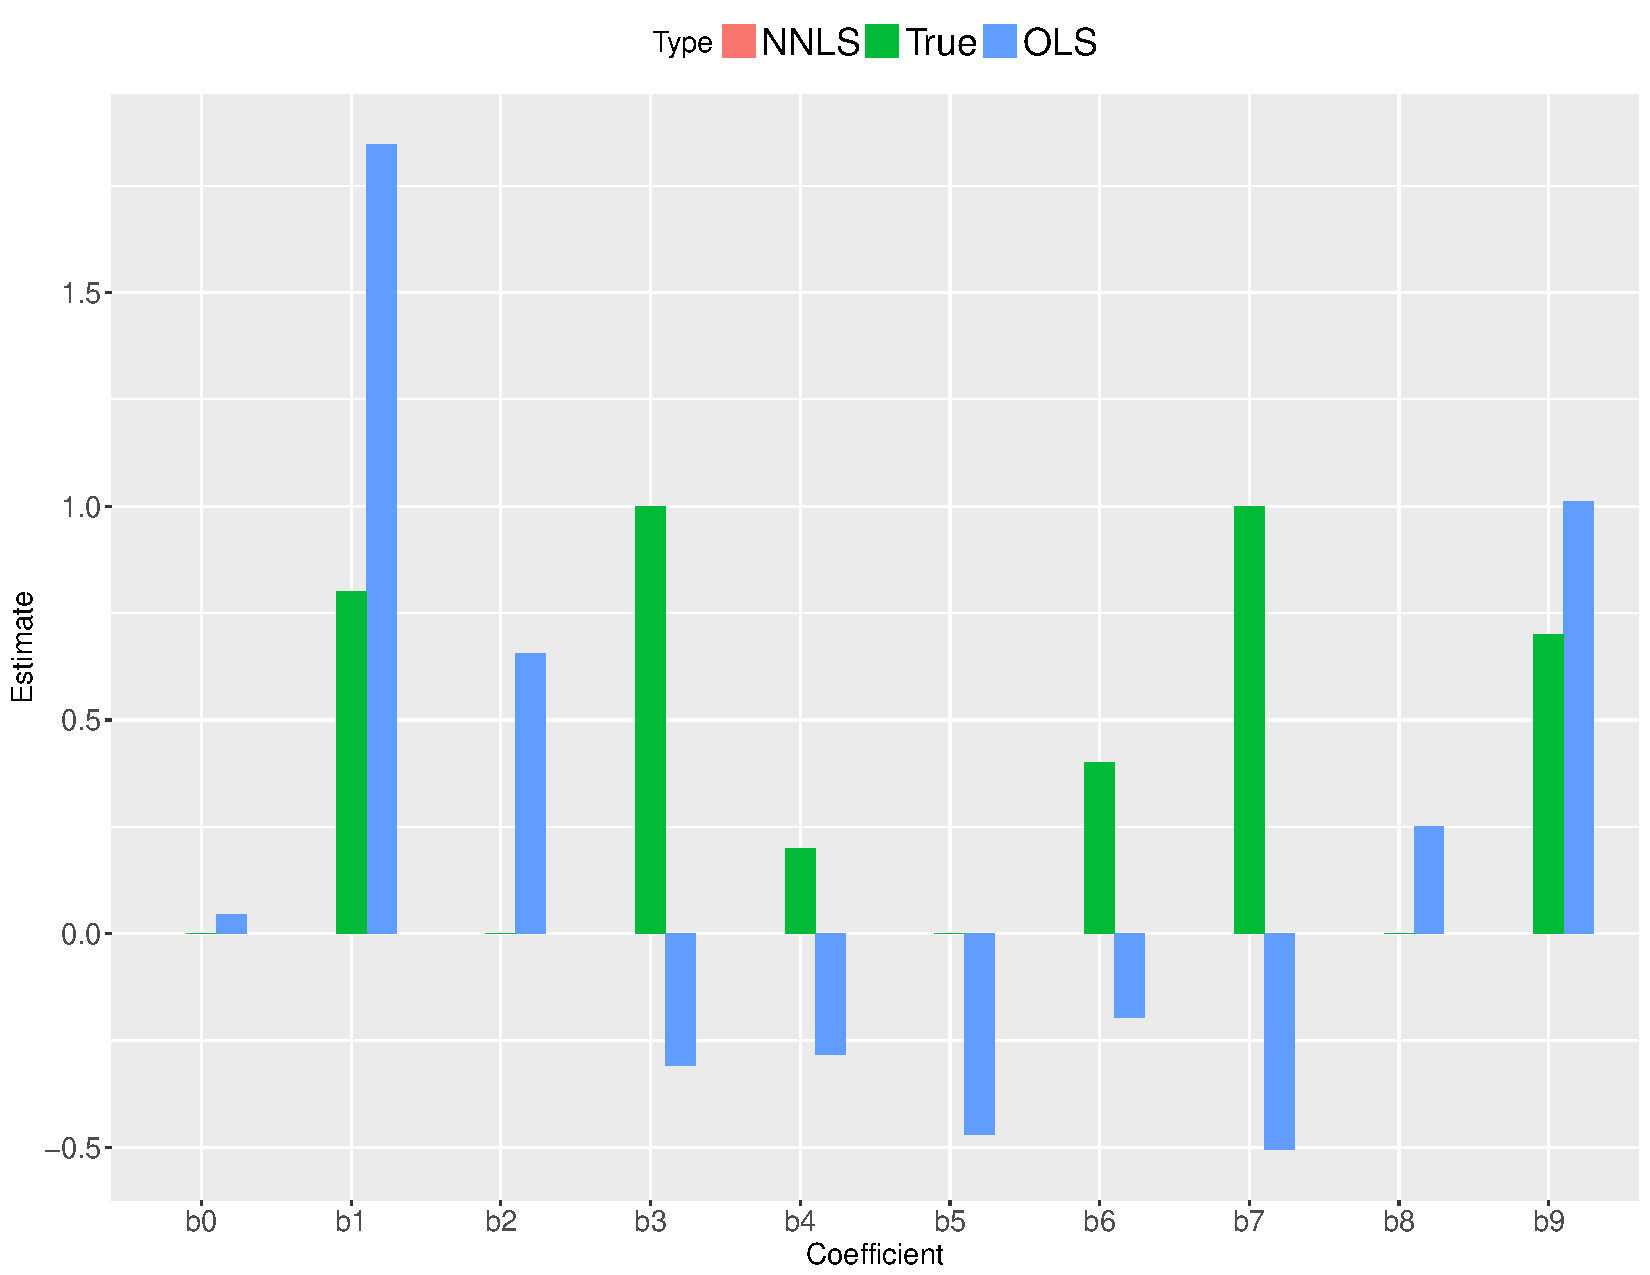
\includegraphics[width=0.9\textwidth]{figs/nnls1.pdf}
	\end{figure}
	\vfill
\end{frame}

\begin{frame}{True vs. Estimated Coefficients}
	\vfill
	\begin{figure}
		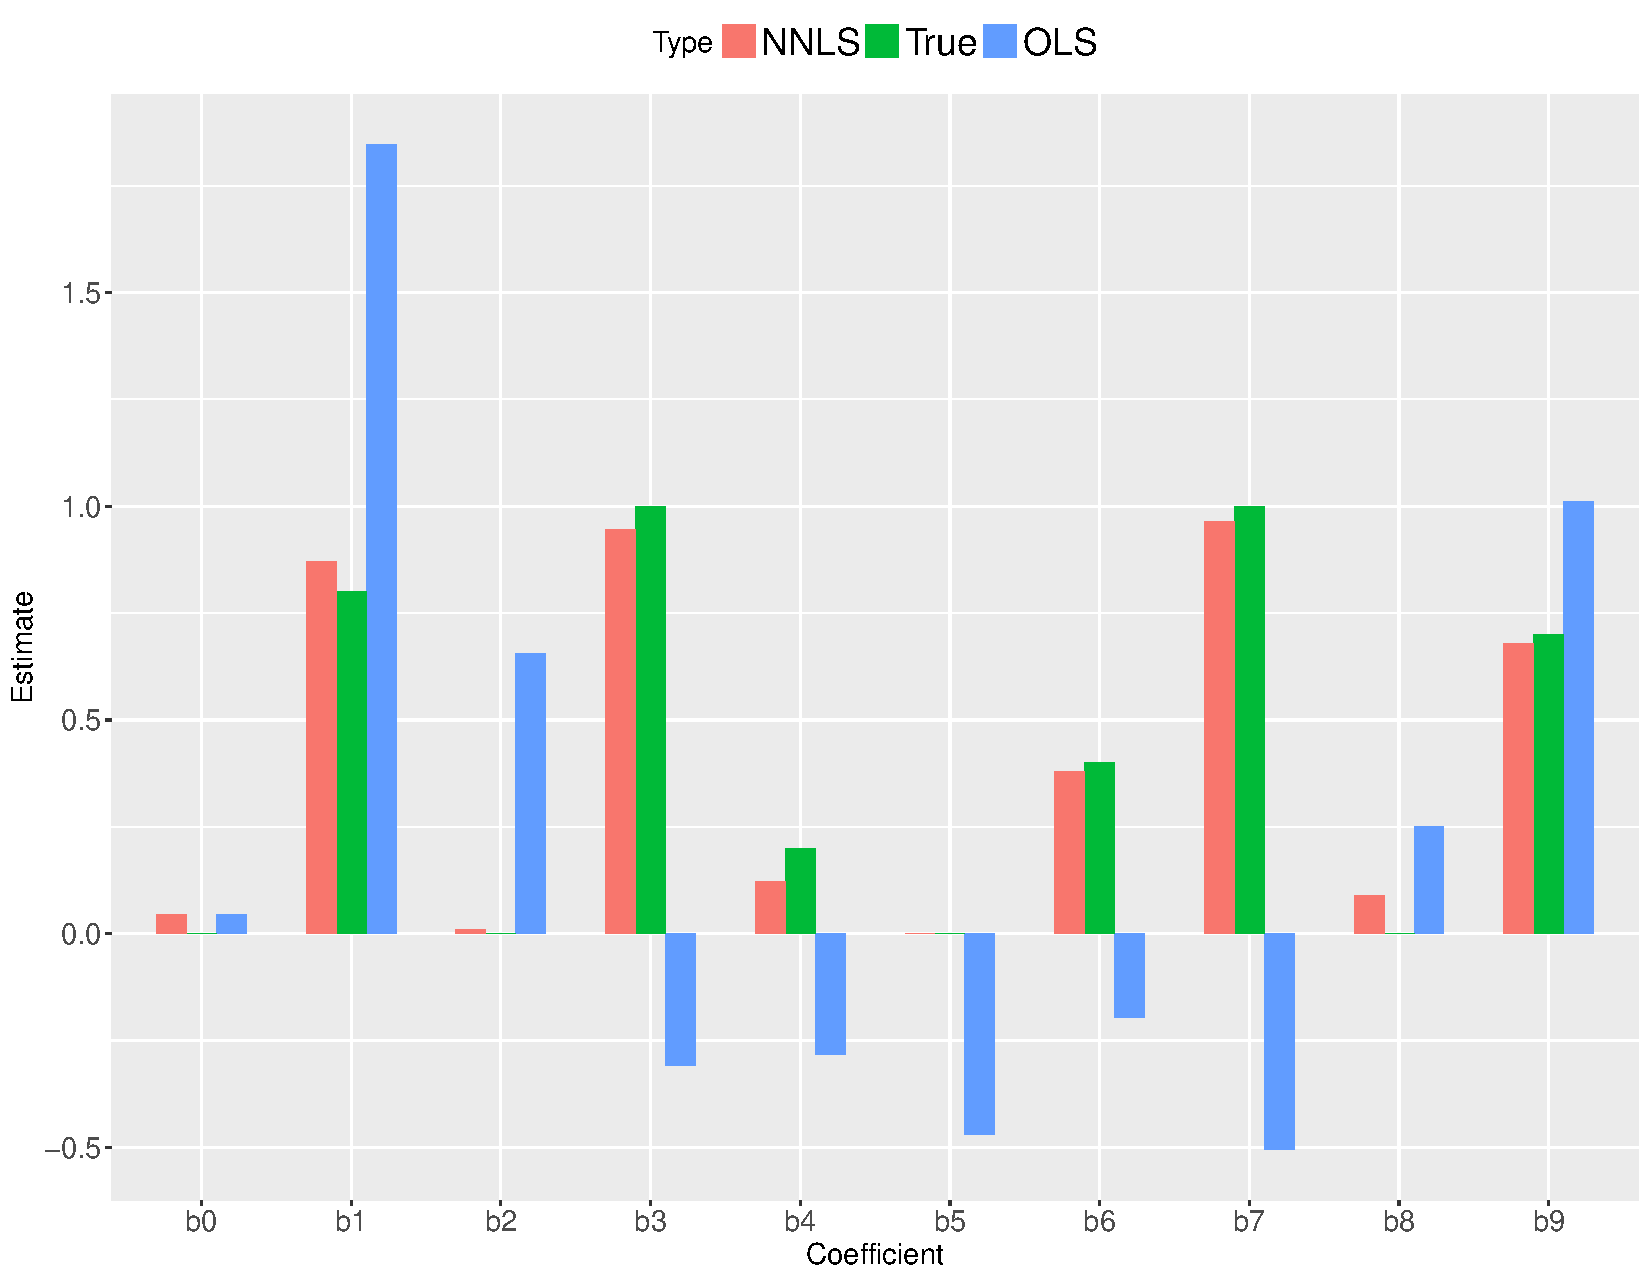
\includegraphics[width=0.9\textwidth]{figs/nnls2.pdf}
	\end{figure}
	\vfill
\end{frame}

\iffalse
\begin{frame}{Direct Standardization}
	% Given non-uniform samples $X,y$ and known expectations for features in $X$, guess distribution of $y$
	\BIT
		\item Samples $(X,y)$ drawn \textbf{non-uniformly} from a distribution
		\item Expectations of columns of $X$ have known values $b \in \reals^n$
		
		\pause
		\item Empirical distribution $y = y_i$ w.p. $1/m$ is \textbf{not} a good estimate of distribution of $y$
		\item Let's use weighted empirical distribution $y = y_i$ w.p. $w_i$
		% \item Let's weight the samples with $w = (w_1,\ldots,w_n)$
		\item Choose $w = (w_1,\ldots,w_m)$ to match known expectations, 
maximize entropy
	\EIT
	
	\[
	\begin{array}{ll} \mbox{maximize} & \sum_i^m -w_i \log w_i \\
	\mbox{subject to} & w \geq 0 \quad \ones^Tw = 1 \quad X^Tw = b
	\end{array}
	\]
\end{frame}
\fi

\iffalse
\begin{frame}[fragile]{Direct Standardization}
	\begin{verbatim}
	w <- Variable(m)
	obj <- sum(entr(w))
	constr <- list(w >= 0, sum(w) == 1, t(X) %*% w == b)
	prob <- Problem(Maximize(obj), constr)
	result <- solve(prob)
	result$getValue(w)
	\end{verbatim}
	
	\BIT
		\item \verb|entr| is the elementwise entropy function
		\item \verb|result$getValue(w)| returns an R vector of weights
	\EIT
\end{frame}
\fi

\iffalse
\begin{frame}{True vs. Sample Probability Distribution}
	\vfill
	\begin{figure}
		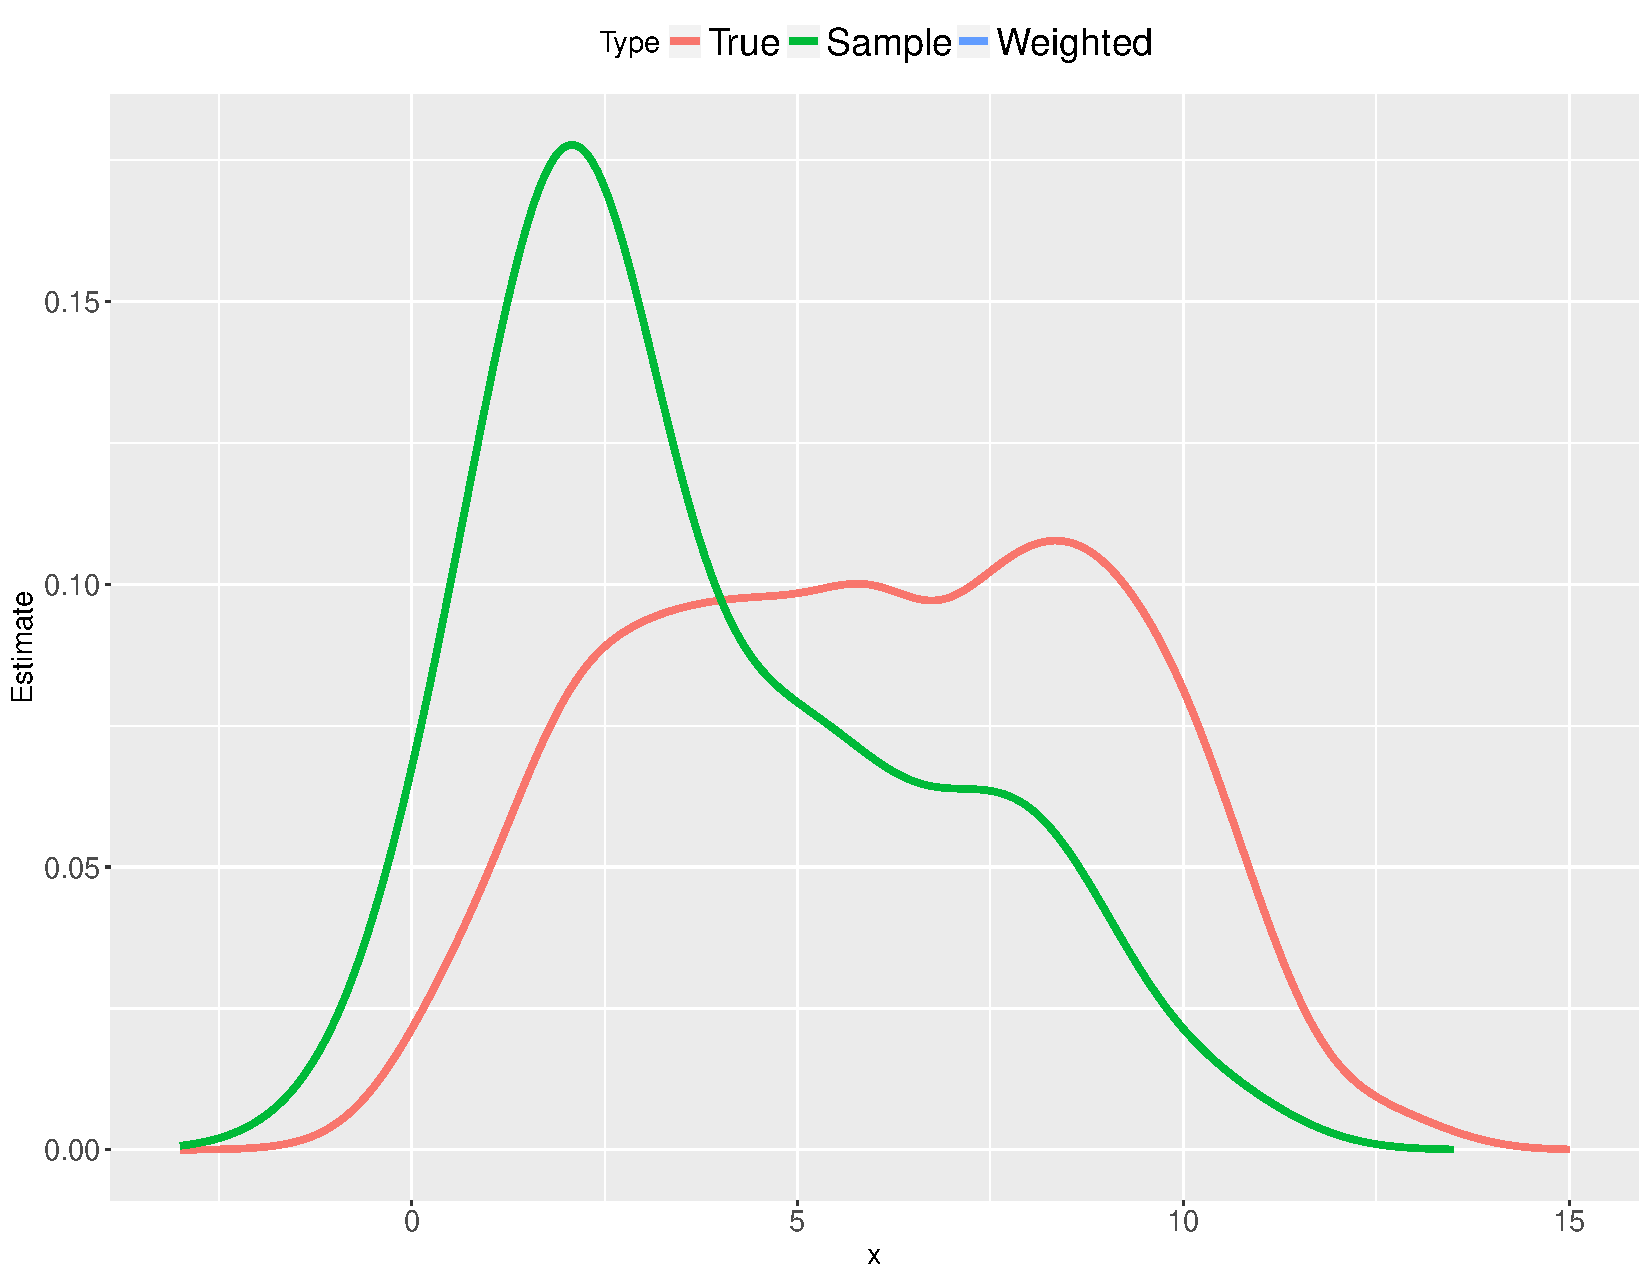
\includegraphics[width=0.9\textwidth]{figs/dstand_pdf1.pdf}
	\end{figure}
	\vfill
\end{frame}
\fi

\iffalse
\begin{frame}{True vs. Weighted Probability Distribution}
	\vfill
	\begin{figure}
		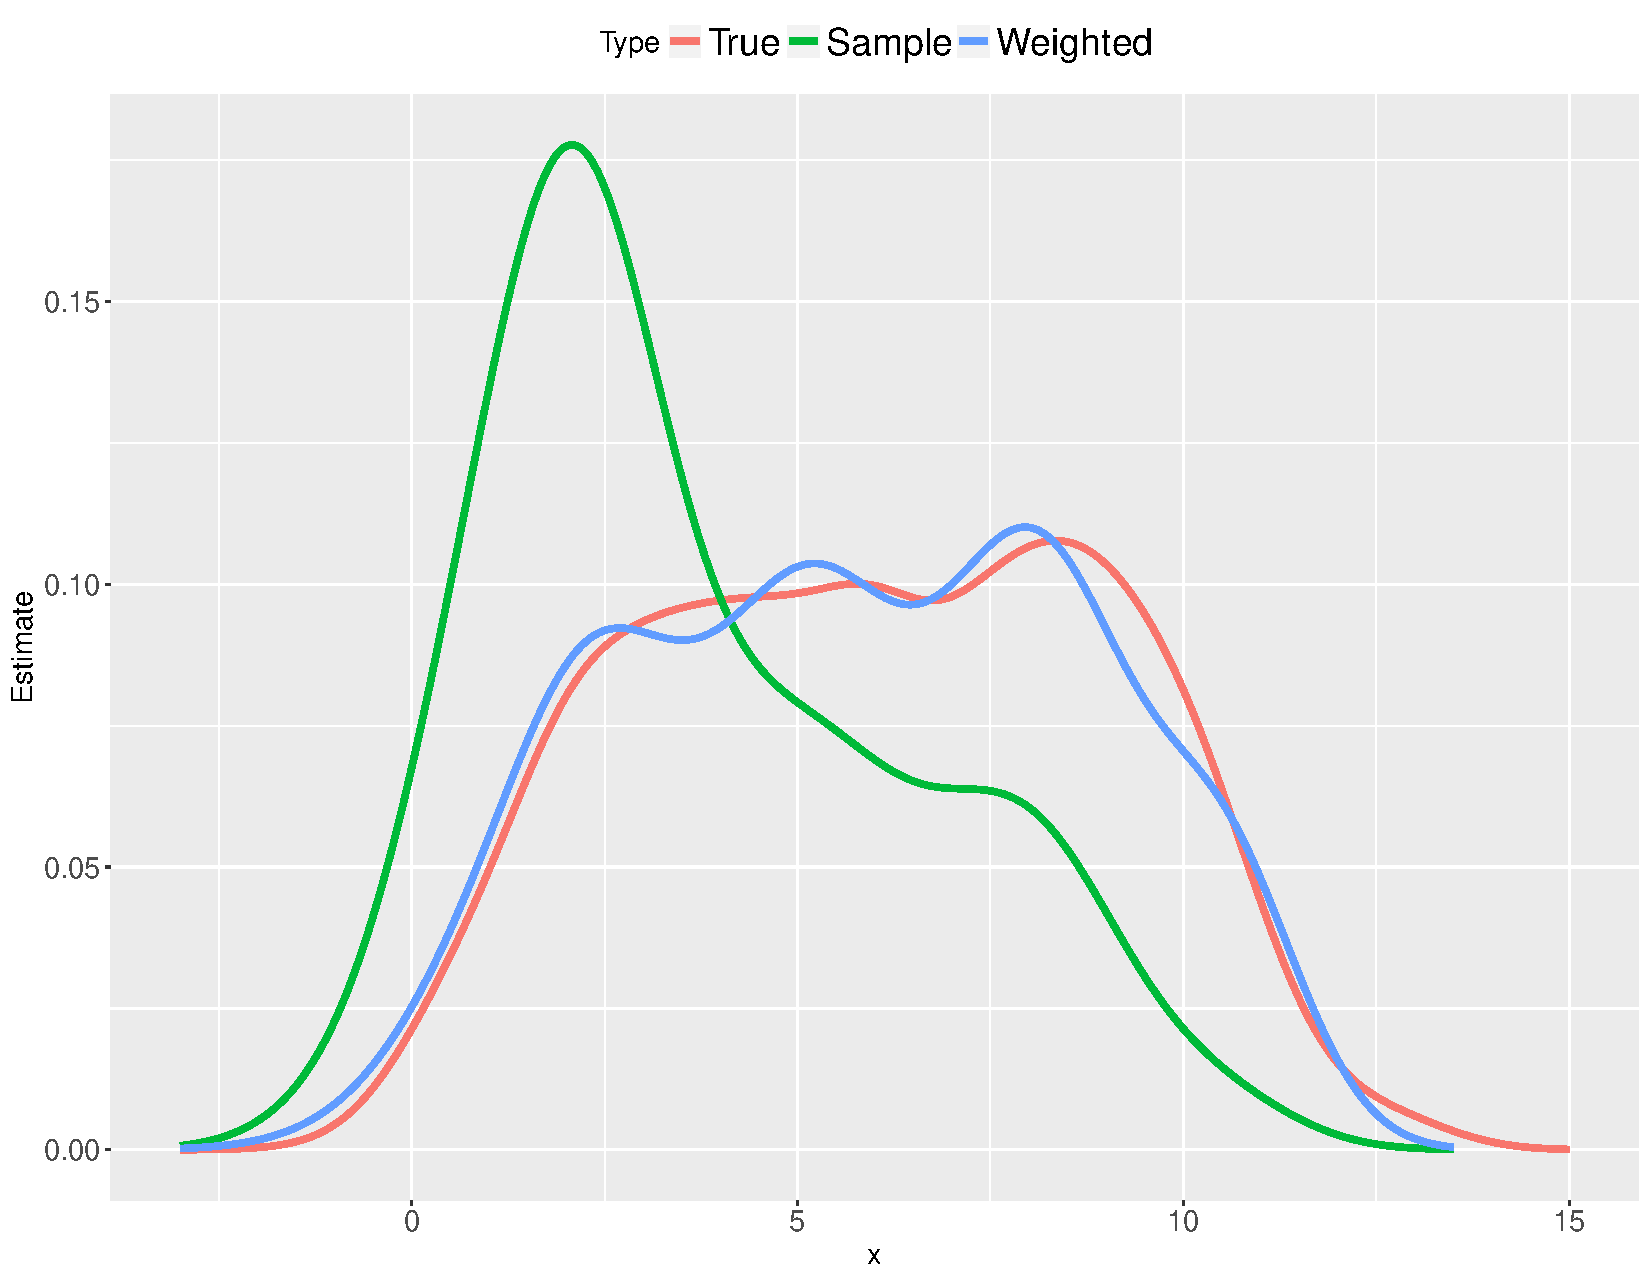
\includegraphics[width=0.9\textwidth]{figs/dstand_pdf2.pdf}
	\end{figure}
	\vfill
\end{frame}
\fi

\iffalse
\begin{frame}{True vs. Estimated Cumulative Distribution}
	\vfill
	\begin{figure}
		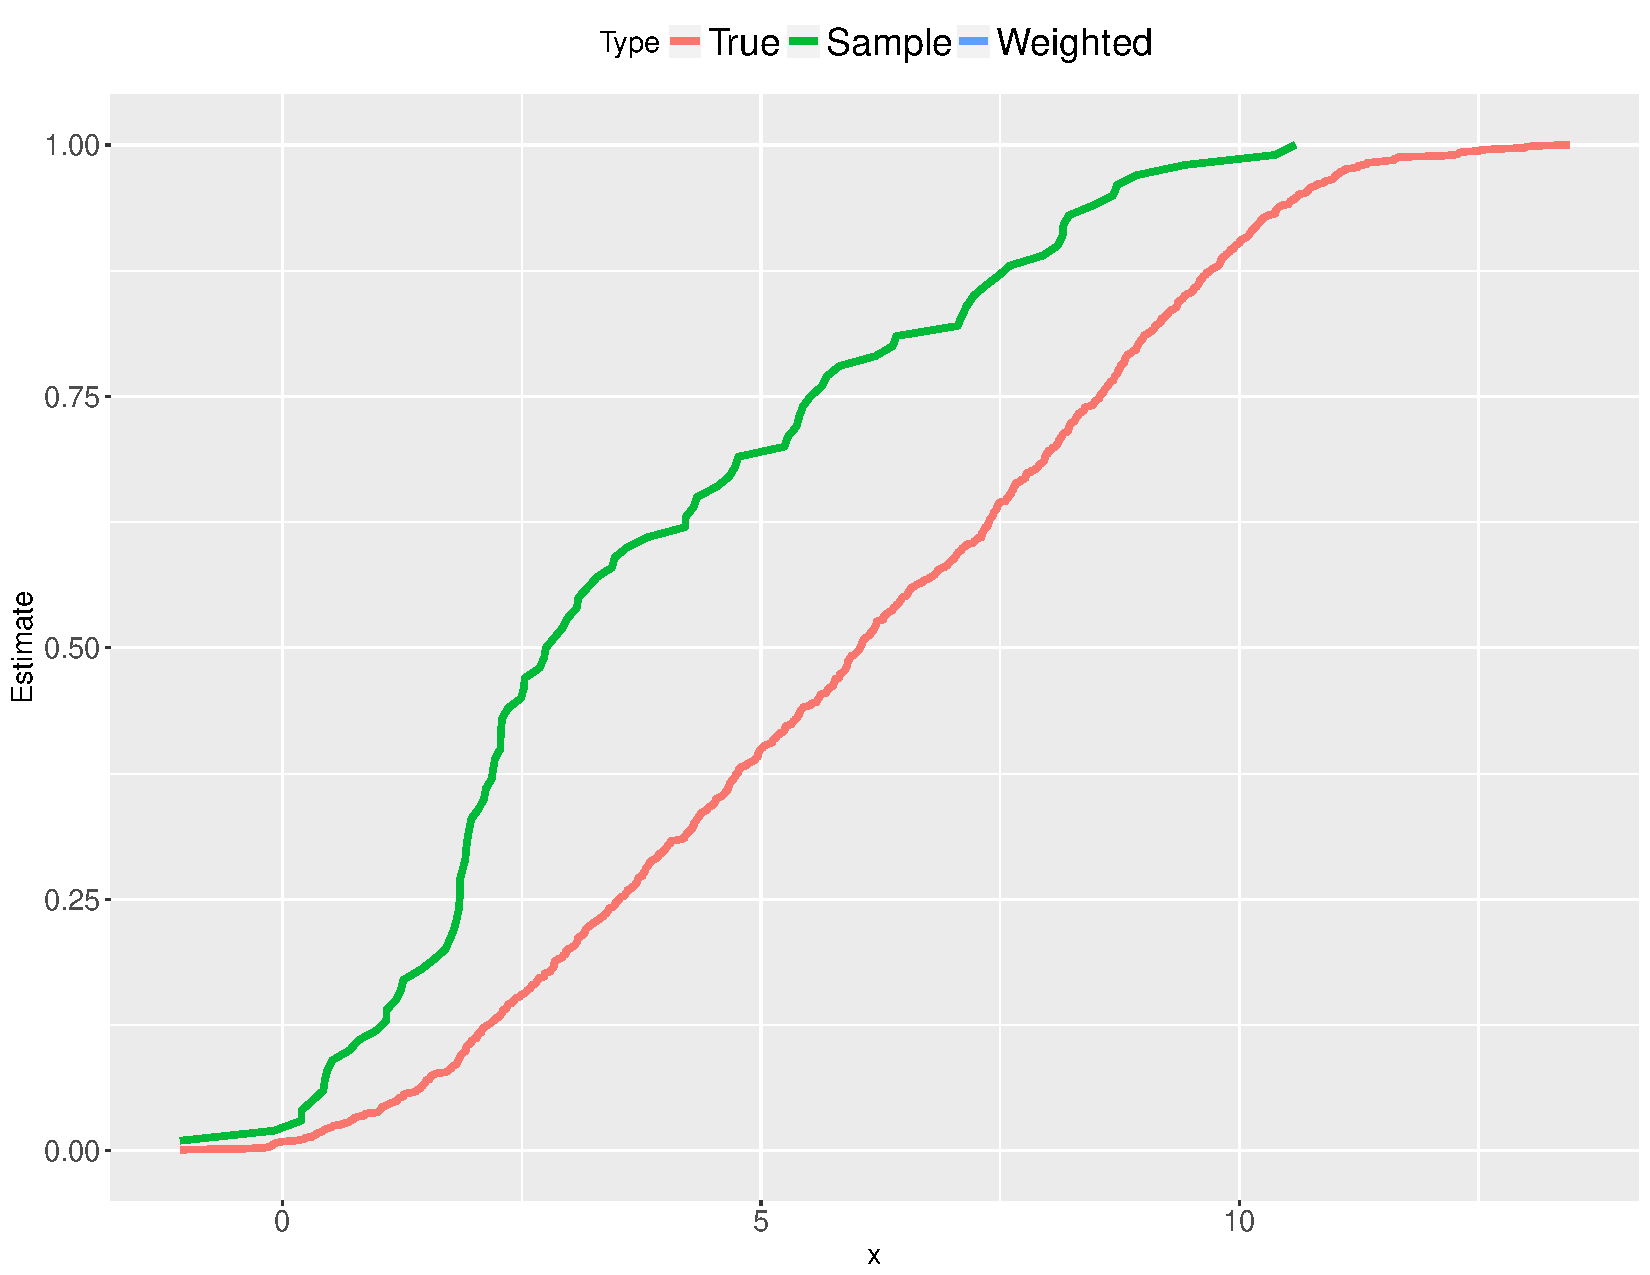
\includegraphics[width=0.9\textwidth]{figs/dstand_cdf1.pdf}
	\end{figure}
	\vfill
\end{frame}
\fi

\iffalse
\begin{frame}{True vs. Estimated Cumulative Distribution}
	\vfill
	\begin{figure}
		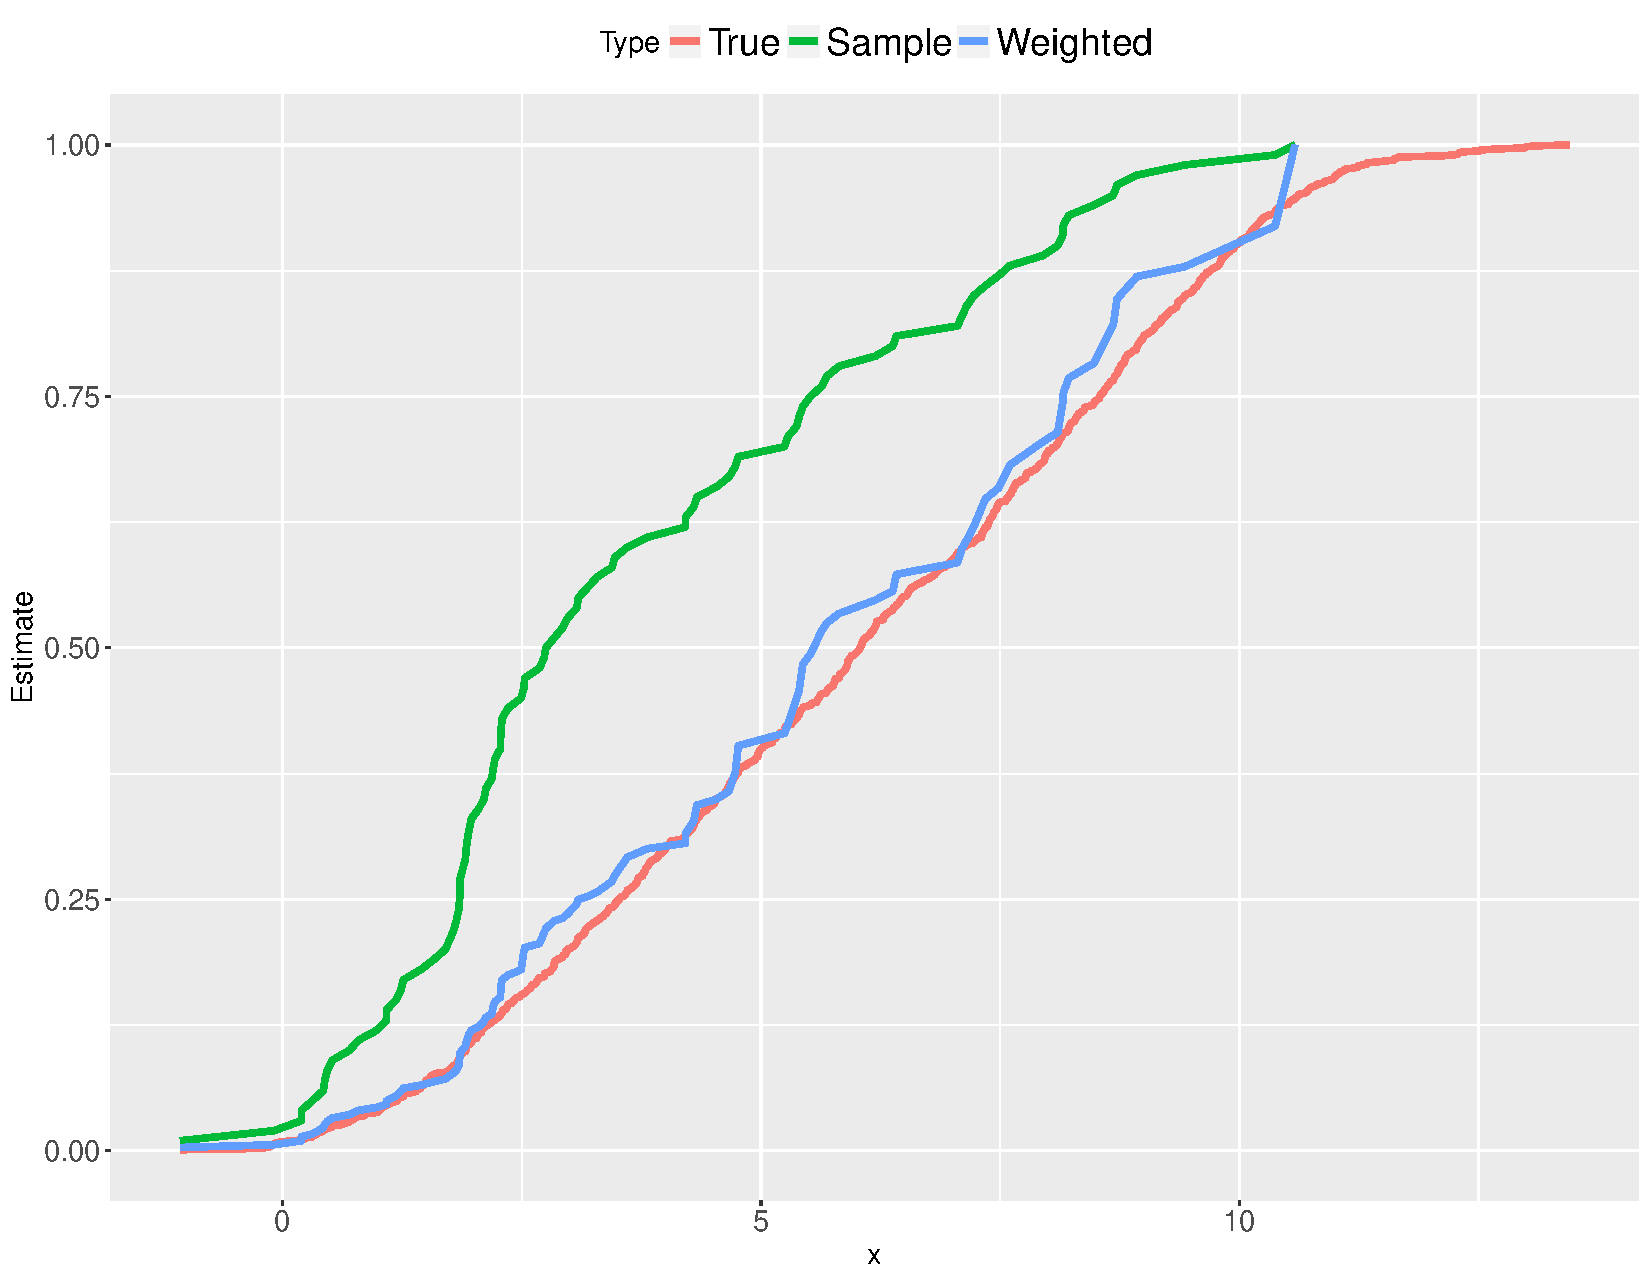
\includegraphics[width=0.9\textwidth]{figs/dstand_cdf2.pdf}
	\end{figure}
	\vfill
\end{frame}
\fi

\begin{frame}{Fastest Mixing Markov Chain}
	\BIT
		\item TODO: Set up FMMC problem
	\EIT
	
	\[
	\begin{array}{ll} \mbox{minimize} & \lambda_{\max}(P - \frac{1}{n}\ones\ones^{\top}) \\
	\mbox{subject to} & P \geq 0, \quad P\ones = \ones, \quad P = P^{\top} \\
	& P_{ij} = 0, \quad (i,j) \notin \mathcal{E}
	\end{array}
	\]
\end{frame}

\begin{frame}[fragile]{Fastest Mixing Markov Chain}
	\begin{verbatim}
	P <- Variable(n,n)
	obj <- Minimize(lambda_max(P - 1/n))
	constr <- list(P >= 0, P %*% ones == ones, P == t(P), 
	+    P[idxs] == 0)
	prob <- Problem(obj, constr)
	result <- solve(prob)
	result$getValue(P)
	\end{verbatim}
	
	\BIT
		\item \verb|lambda_max| is the maximum eigenvalue function (can also use spectral norm)
		\item \verb|idxs| is matrix containing all unconnected vertices $(i,j)$
	\EIT
\end{frame}

\begin{frame}{Triangle + 1 Edge}
	\vfill
	\begin{figure}
		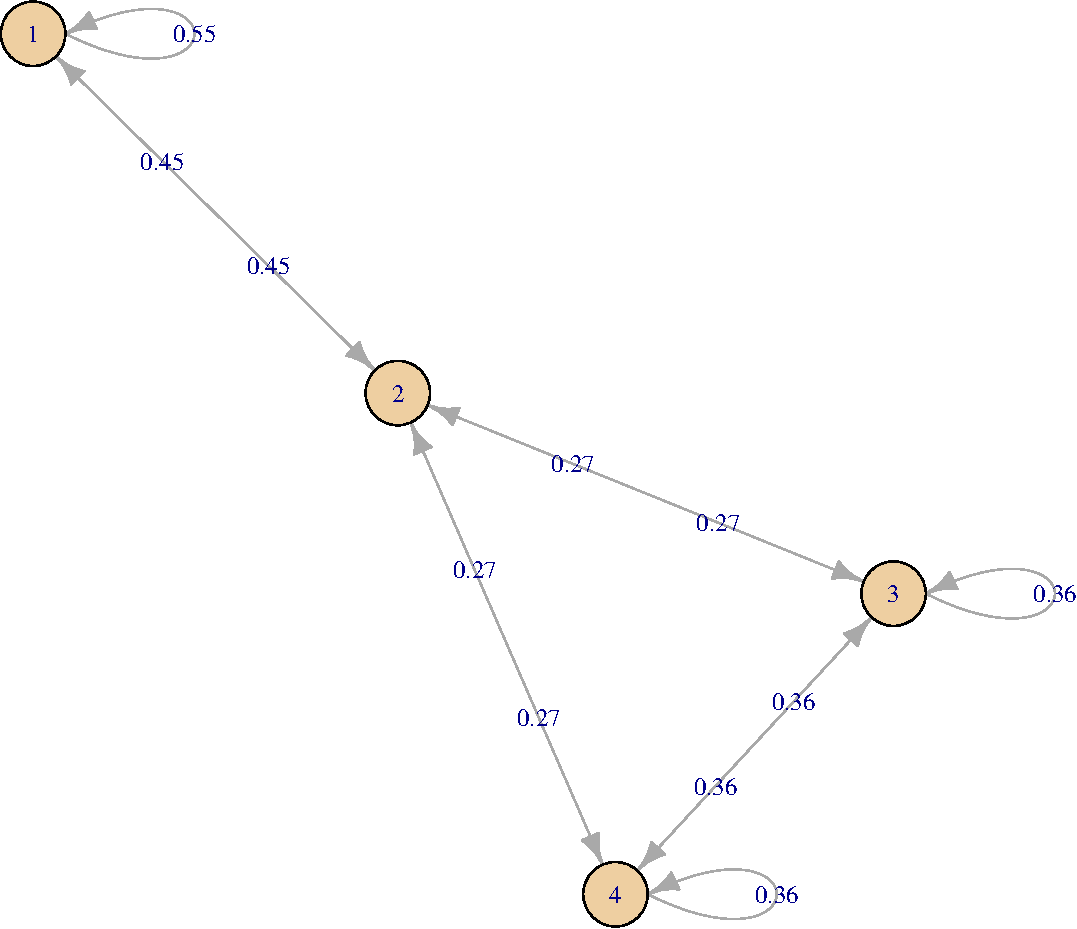
\includegraphics[width=0.8\textwidth]{figs/fmmc_triangle.pdf}
	\end{figure}
	\vfill
\end{frame}

\begin{frame}{Bipartite 2 + 3}
	\vfill
	\begin{figure}
		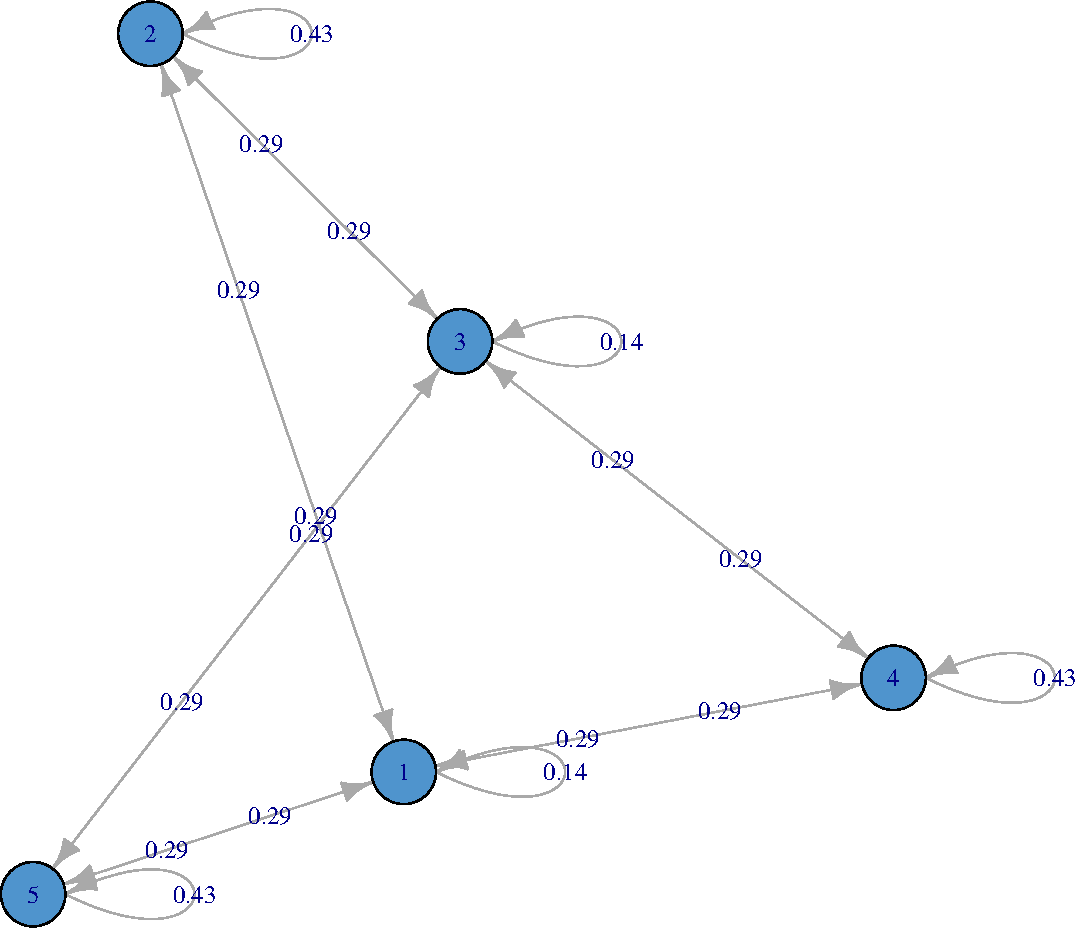
\includegraphics[width=0.8\textwidth]{figs/fmmc_bipartite.pdf}
	\end{figure}
	\vfill
\end{frame}

%\section{Disciplined Convex Programming}

\iffalse
\begin{frame}{Curvature: Convex, Concave, and Affine functions}
	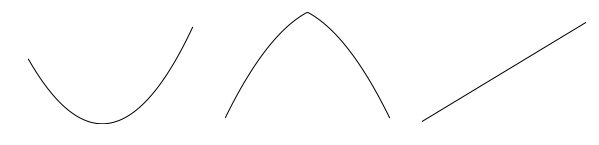
\includegraphics[width=0.9\textwidth,height=0.20\textheight]{figs/curvature.png}
	\BIT
		\item $f$ is \emph{concave} if $-f$ is convex, \ie, for any $x,y$,
		$\theta \in [0,1]$,
		\[
		f(\theta x + (1-\theta) y) \geq \theta f(x) + (1-\theta) f(y)
		\]
		\item $f$ is \emph{affine} if it is convex and concave, \ie,
		\[
		f(\theta x + (1-\theta) y) = \theta f(x) + (1-\theta) f(y)
		\]
		for any $x,y$, $\theta \in [0,1]$
		\item $f$ is affine $\Longleftrightarrow$ it has form
		$f(x) = a^Tx +b$
	\EIT
\end{frame}
\fi

\iffalse
\begin{frame}{Verifying a Function is Convex or Concave}
	(Verifying affine is easy)
	
	\vfill
	Approaches:
	\BIT
		\item Via basic definition (inequality)
		\item Via first or second order conditions, \eg, $\nabla^2 f(x) \succeq 0$
		
		\vfill
		
		\item Via convex calculus: construct $f$ using
		\BIT
			\item Library of basic functions that are convex or concave
			\item Calculus rules or transformations that preserve convexity
		\EIT
	\EIT
\end{frame}
\fi

\iffalse
\begin{frame}{Disciplined Convex Programming (DCP)}
	(\emph{Grant, Boyd, Ye, 2006})
	
	\vfill
	\BIT
		\item Framework for describing convex optimization problems
		\item Based on constructive convex analysis
		\item Sufficient, but not necessary for convexity
		\item Basis for several domain-specific languages and tools for convex optimization
		\BIT
			\item CVX, YALMIP, CVXPY, Convex.jl
		\EIT
	\EIT
	\vfill
\end{frame}
\fi

\section{Future Work}
\begin{frame}{Future Work}
	\BIT
		\item Flesh out convex functions in library
		\item Develop more applications and examples
		\item Add warm start support
		\item Further speed improvements
	\EIT
	
	Official site: \url{cvxr.rbind.io} \\
	CRAN page: \url{CRAN.R-project.org/package=CVXR}
\end{frame}

\end{document}
